\documentclass[aspectratio=169]{beamer}
\usepackage[utf8]{inputenc}
\usepackage{lmodern}
\usepackage{tikz}
\usepackage{hyperref}
\usetikzlibrary{positioning,arrows.meta,calc}

\definecolor{accent1}{HTML}{2D6A4F}
\definecolor{accent2}{HTML}{95D5B2}
\definecolor{accent3}{HTML}{F4A261}
\definecolor{accent4}{HTML}{1B4332}
\definecolor{paper}{HTML}{F7FFF7}
\definecolor{ink}{HTML}{1F2937}

\setbeamertemplate{navigation symbols}{}
\setbeamercolor{normal text}{fg=ink,bg=white}
\setbeamercolor{frametitle}{fg=ink,bg=white}
\setbeamertemplate{itemize item}{\color{accent1}$\blacktriangleright$}
\setbeamertemplate{enumerate item}{\color{accent1}\insertenumlabel.}
\setbeameroption{hide notes}

\title{Minecraft: Windmill}
\subtitle{Student Guide}
\author{Pine Brook IGNITE}
\date{Spring 2026}

\begin{document}

\begin{frame}[plain]
\begin{tikzpicture}[remember picture,overlay]
\fill[paper] (current page.south west) rectangle (current page.north east);
\fill[accent1!10] (0.25,0.4) rectangle (13.05,7.0);
\draw[line width=7pt, color=accent3] (0.55,6.75) -- (12.75,6.75);
\draw[line width=7pt, color=accent2] (0.55,0.65) -- (12.75,0.65);
\end{tikzpicture}
\vspace{0.45cm}
\begin{columns}[T,totalwidth=\textwidth]
\column{0.56\textwidth}
{\huge\bfseries\color{ink} Minecraft: Windmill\par}
\vspace{0.2cm}
{\Large\color{accent4} Build. Code. Test.\par}
\vspace{0.25cm}

\begin{tikzpicture}
\node[rounded corners=16pt, fill=white, draw=accent1, line width=1.2pt, text width=6.2cm, minimum height=1.35cm, align=center]
{\Large\bfseries Build and code your way through a Minecraft challenge.};
\end{tikzpicture}
\vspace{0.35cm}
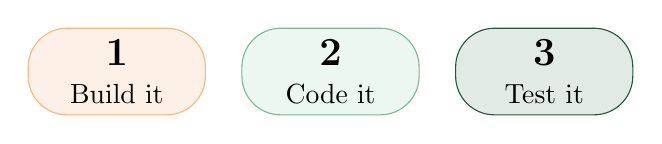
\begin{tikzpicture}[node distance=0.45cm]
\node[rounded corners=14pt, fill=accent3!16, draw=accent3!80, minimum width=2.25cm, minimum height=1.1cm, align=center] (a) {\Large\bfseries 1\\[2pt]Build it};
\node[rounded corners=14pt, fill=accent2!18, draw=accent2!85!black, minimum width=2.25cm, minimum height=1.1cm, align=center, right=of a] (b) {\Large\bfseries 2\\[2pt]Code it};
\node[rounded corners=14pt, fill=accent1!14, draw=accent1!80!black, minimum width=2.25cm, minimum height=1.1cm, align=center, right=of b] (c) {\Large\bfseries 3\\[2pt]Test it};
\end{tikzpicture}
\column{0.4\textwidth}
\begin{center}

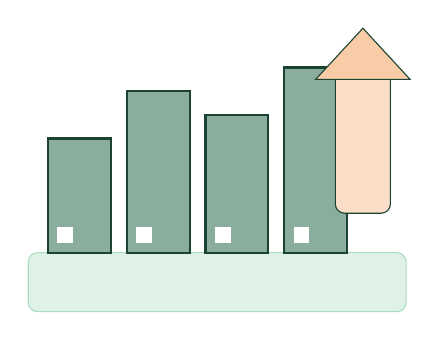
\begin{tikzpicture}[x=1cm,y=1cm]
\draw[rounded corners=0.12cm, fill=accent2!30, draw=accent2!80] (0.1,0.15) rectangle (4.9,0.9);
\foreach \x/\h in {0.35/1.45,1.35/2.05,2.35/1.75,3.35/2.35} {
  \draw[fill=accent1!55, draw=accent4, line width=0.8pt] (\x,0.9) rectangle ++(0.8,\h);
  \draw[fill=white!18, draw=none] (\x+0.12,1.02) rectangle ++(0.2,0.2);
}
\draw[fill=accent3!35, draw=accent4, rounded corners=0.12cm] (4.0,1.4) rectangle (4.7,3.4);
\draw[fill=accent3!55, draw=accent4] (3.75,3.1) -- (4.35,3.75) -- (4.95,3.1) -- cycle;
\end{tikzpicture}

\end{center}
\end{columns}
\note{Audience guidance: Intermediate learners who can handle complex digital tasks when setup friction, debugging, and persistence are explicitly. Teaching move: Project the exact click path before students begin so setup friction does not consume}
\end{frame}

\begin{frame}[plain]
\frametitle{Today's Mission}
\begin{columns}[T,totalwidth=\textwidth]
\column{0.56\textwidth}
\begin{block}{Our focus}
\normalsize Use Minecraft code to solve a build challenge.
\end{block}
\vspace{0.1cm}
\begin{itemize}
\normalsize
\item Student completes the core task or an accessible version
\item Student can explain at least one step, pattern, choice,
\item Teacher captures one proof item: screenshot, observation note, exit
\end{itemize}
\column{0.38\textwidth}
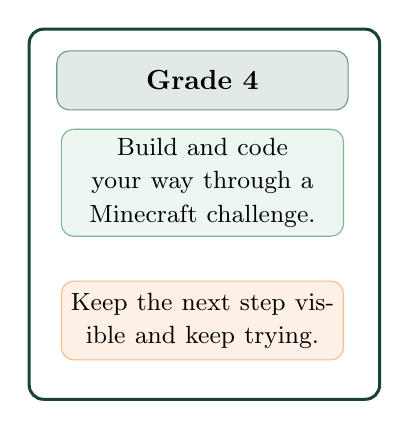
\begin{tikzpicture}[x=1cm,y=1cm]
\draw[rounded corners=0.18cm, fill=white, draw=accent4, line width=1.1pt] (0.1,0.1) rectangle (4.55,4.8);
\node[rounded corners=0.16cm, fill=accent1!14, draw=accent1!70, minimum width=3.7cm, minimum height=0.75cm, align=center] at (2.3,4.15) {\bfseries Grade 4};
\node[rounded corners=0.16cm, fill=accent2!18, draw=accent2!85!black, text width=3.35cm, minimum height=1.2cm, align=center] at (2.3,2.85) {\small Build and code your way through a Minecraft challenge.};
\node[rounded corners=0.16cm, fill=accent3!16, draw=accent3!75, text width=3.35cm, minimum height=1.0cm, align=center] at (2.3,1.1) {\small Keep the next step visible and keep trying.};
\end{tikzpicture}
\end{columns}
\note{Open with the mission in student language. Keep the focus visible while students work.} 
\end{frame}

\begin{frame}[plain]
\frametitle{How We Will Move Through It}
\begin{center}
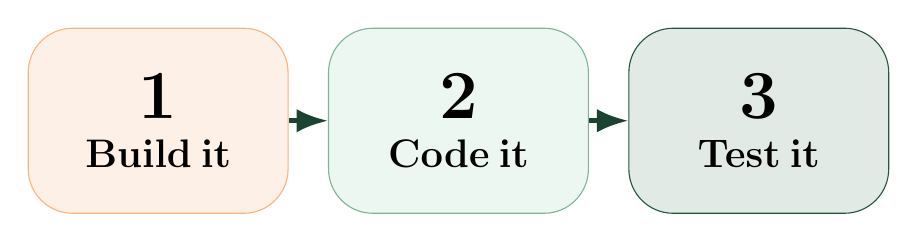
\begin{tikzpicture}[node distance=0.5cm]
\node[rounded corners=16pt, fill=accent3!16, draw=accent3!80, minimum width=3.3cm, minimum height=2.35cm, text width=2.45cm, align=center] (s1) {\Huge\bfseries 1\\[6pt]\Large Build it};
\node[rounded corners=16pt, fill=accent2!18, draw=accent2!85!black, minimum width=3.3cm, minimum height=2.35cm, text width=2.45cm, align=center, right=of s1] (s2) {\Huge\bfseries 2\\[6pt]\Large Code it};
\node[rounded corners=16pt, fill=accent1!14, draw=accent1!80!black, minimum width=3.3cm, minimum height=2.35cm, text width=2.45cm, align=center, right=of s2] (s3) {\Huge\bfseries 3\\[6pt]\Large Test it};
\draw[-{Latex[length=4mm,width=3mm]}, line width=1.7pt, color=accent4] (s1) -- (s2);
\draw[-{Latex[length=4mm,width=3mm]}, line width=1.7pt, color=accent4] (s2) -- (s3);
\end{tikzpicture}
\end{center}
\vspace{0.25cm}
\begin{block}{What to keep in front of you}
\begin{itemize}
\normalsize
\item Model the first step before independent or partner work starts.
\item Keep one visible checklist, anchor chart, or projected example available throughout
\item Pause once mid-lesson for a quick debug, reflection, or reset point.
\end{itemize}
\end{block}
\note{Keep this slide up during work time when students need a visible routine.} 
\end{frame}

\begin{frame}[plain]
\frametitle{If You Get Stuck}
\begin{columns}[T,totalwidth=\textwidth]
\column{0.5\textwidth}
\begin{block}{Use this help ladder}
\begin{enumerate}
\normalsize
\item Look at the slide.
\item Try one small step.
\item Ask your partner.
\item Ask one clear question.
\end{enumerate}
\end{block}
\column{0.45\textwidth}
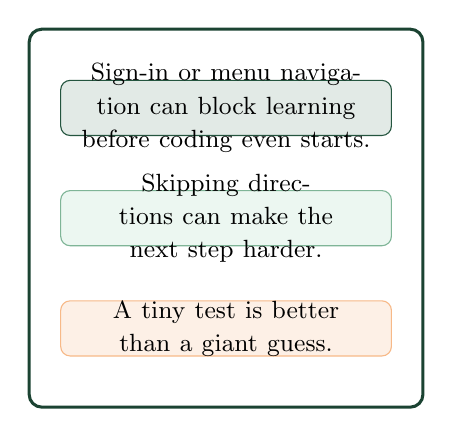
\begin{tikzpicture}[x=1cm,y=1cm]
\draw[rounded corners=0.16cm, fill=white, draw=accent4, line width=1.1pt] (0.0,0.0) rectangle (5.0,4.8);
\draw[rounded corners=0.12cm, fill=accent1!14, draw=accent1!80!black] (0.4,3.45) rectangle (4.6,4.15);
\node[text width=3.7cm, align=center] at (2.5,3.8) {\small Sign-in or menu navigation can block learning before coding even starts.};
\draw[rounded corners=0.12cm, fill=accent2!18, draw=accent2!85!black] (0.4,2.05) rectangle (4.6,2.75);
\node[text width=3.7cm, align=center] at (2.5,2.4) {\small Skipping directions can make the next step harder.};
\draw[rounded corners=0.12cm, fill=accent3!16, draw=accent3!75] (0.4,0.65) rectangle (4.6,1.35);
\node[text width=3.7cm, align=center] at (2.5,1.0) {\small A tiny test is better than a giant guess.};
\end{tikzpicture}
\end{columns}
\note{Name the next small move. Hints before rescues.} 
\end{frame}

\begin{frame}[plain]
\frametitle{Show What You Learned}
\begin{center}
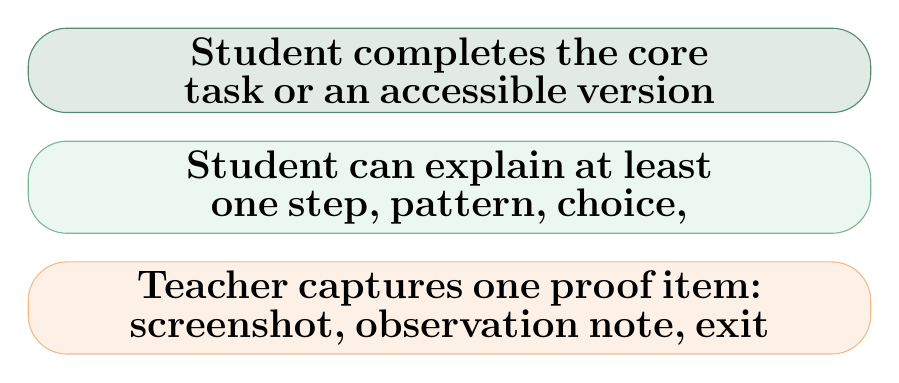
\begin{tikzpicture}[node distance=0.35cm]
\node[rounded corners=14pt, fill=accent1!14, draw=accent1!80, minimum width=10.7cm, minimum height=1.0cm, text width=9.5cm, align=center] (a) {\Large\bfseries Student completes the core task or an accessible version};
\node[rounded corners=14pt, fill=accent2!18, draw=accent2!85!black, minimum width=10.7cm, minimum height=1.0cm, text width=9.5cm, align=center, below=of a] (b) {\Large\bfseries Student can explain at least one step, pattern, choice,};
\node[rounded corners=14pt, fill=accent3!16, draw=accent3!75, minimum width=10.7cm, minimum height=1.0cm, text width=9.5cm, align=center, below=of b] (c) {\Large\bfseries Teacher captures one proof item: screenshot, observation note, exit};
\end{tikzpicture}
\end{center}
\vspace{0.28cm}
\begin{block}{Finish strong}
\Large Save it, share it, explain it, or demonstrate it.
\end{block}
\note{Close with one visible proof move and one clear celebration cue.}
\end{frame}

\end{document}
